\documentclass[10pt]{article}
\usepackage[utf8x]{inputenc}
\usepackage{polski}

\usepackage{amsmath}
\usepackage{amsthm}
\usepackage{amssymb}

\usepackage{graphics}
\usepackage{pdfpages}
\DeclareGraphicsRule{.1}{mps}{*}{}
\usepackage{epstopdf}

\usepackage{geometry}
\geometry{a4paper, margin=2cm}

\begin{document}
    
%NAGLOWEK

    \noindent
    \begin{minipage}{0.5\textwidth}
        \LARGE{\textsf{\textbf{Zadanie: STR\\Strażnicy}}}
    \end{minipage}
    \begin{minipage}{0.5\textwidth}
        \begin{flushright}
            
\includegraphics[height=1.5cm]{logo.jpg}
        \end{flushright}
    \end{minipage}
    
    \noindent\rule{\textwidth}{0.4pt}
    
    \noindent\textbf{Akademia Programowania PWSW, dzień V, Dostępna pamięć: 128 MB.}
    \vspace{1em}
    
%TRESC
    
    \noindent
    Bajtocka Galeria Narodowa, która składa się z pewnej liczby sal oraz łączących je korytarzy (z każdej sali da się dojść do wszystkich pozostałych), posiada w swojej kolekcji wiele unikatowych przedmiotów. Dlatego aby chronić zebrane przedmioty, dyrektor galerii postanowił zatrudnić strażników. Każdy z zatrudnionych strażników zostanie przypisany do pewnej sali i będzie obserwował co najwyżej dwa wychodzące z niej korytarze. Dyrektor chce mieć pewność, że nikt nie będzie przemieszczał się między salami, dlatego zatrudni tylu strażników, aby każdy z korytarzy był obserwowany przez co najmniej jednego strażnika.
    
    Ponieważ dyrektor nie chce płacić za nadmiarową ochronę (chce zostawić więcej pieniędzy na zakup nowych dzieł do galerii) postanowił zatrudnić Ciebie, aby dowiedzieć się jaka jest minimalna liczba strażników, których powinien zatrudnić i jak powinni zostać oni ustawieni.

%WEJSCIE

    \section*{Wejście}
    
    W pierwszym wierszu standardowego wejścia znajdują się dwie liczby całkowite $n$ i $m$, $(1\leq n, m\leq 200000)$ oznaczające odpowiednio liczbę sal i łączących je korytarzy. W $m$ kolejnych wierszach znajdują się dwie różne liczb całkowitych $u_{i}$ i $v_{i}$ $(1\leq u_{i}, v_{i}\leq n; 1\leq i\leq m)$, oznaczające, że istnieje korytarz łączący sale $u_{i}$ i $v_{i}$, a jego numer to $i$. Każde dwie sale łączy co najwyżej jeden korytarz.

%WYJSCIE

    \section*{Wyjście}
    
    W pierwszym wierszu standardowego wyjścia należy wypisać jedną liczbę całkowitą $s$, oznaczającą liczbę strażników jaką dyrektor powinnien zatrudnić. W kolejnych $s$ wierszach należy wypisać trzy liczby całkowite $r_{i}$, $h_{1_{i}}$, $h_{2_{i}}$, oznaczające odpowiednio numer sali, w której należy ustawić $i$-tego strażnika, oraz numery korytarzy, które ma obserwować ten strażnik. Jeżeli strażnik ma obserwować tylko jeden korytarz, to jako jeden z numerów korytarzy należy wypisać $-1$. Kolejność w jakiej podawane jest ustawienie strażników nie ma znaczenia.

%PRZYKLAD

    \section*{Przykład}
    
    \noindent
    \begin{minipage}[t]{0.5\textwidth}
        Dla danych wejściowych:\vspace{1ex}\\
        \texttt{8 7\\2 3\\2 1\\2 4\\5 2\\4 6\\7 4\\5 8}
    \end{minipage}
    \begin{minipage}[t]{0.5\textwidth}
        poprawnym wynikiem jest:\vspace{1ex}\\
        \texttt{4\\4 5 6\\2 -1 3\\2 1 2\\5 4 7}
    \end{minipage}
    
    \vspace{-2em}
    \begin{center}
        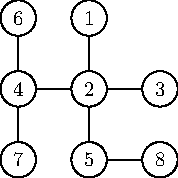
\includegraphics{strrys-1.pdf}
    \end{center}
    
%OCENIANIE

    \section*{Ocenianie}
        
    Zestaw testów dzieli się na następujące podzadania. Testy do każdego podzadania składają się z jednej lub większej liczby osobnych grup testów.
    
    \begin{center}
        \begin{tabular}{ |c|p{9cm}|c| }
            \hline
            \textbf{Podzadanie} & \textbf{Warunki} & \textbf{Liczba punktów}\\
            \hline
            1 & $1\leq n, m\leq 10$ & 15\\
            \hline
            2 & $m = n-1$, galeria jest gąsienicą\footnotemark & 15\\
            \hline
            3 & $m = n-1$ & 25\\
            \hline
            4 & brak dodatkowych ograniczeń & 45\\
            \hline
        \end{tabular}
        \footnotetext{gąsienica - graf, w którym można wyróżnić taką ścieżkę, że każdy liść w grafie jest sąsiedni z pewnym wierzchołkiem ścieżki. Galeria podana jako przykład jest gąsienicą.}
    \end{center}
    
\end{document}
\documentclass[10pt]{article}
\usepackage[utf8x]{inputenc}
\usepackage{polski}

